\documentclass[tikz,openany,11pt,a4paper]{book}
\usepackage{graphicx}
\usepackage[utf8x]{inputenc}
\usepackage{multirow}
\usepackage{blindtext}
\usepackage{graphicx}
\usepackage{numprint}
\usepackage{listings}
\usepackage{xcolor}
\usepackage{amsmath}
\usepackage{mathtools}
\usepackage{float}
\usepackage{caption}
\usepackage{hyperref}
\usepackage{enumitem}
\usepackage{newtxtext,newtxmath}
\usepackage[square,sort,comma,numbers]{natbib}
\usepackage[a4paper, margin=1.5cm]{geometry}
\usepackage{tkz-euclide}
\usepackage{pgfplots}
\author{Metalhead33}
\title{World of Artograch Ruleset}

\definecolor{mGreen}{rgb}{0,0.6,0}
\definecolor{mGray}{rgb}{0.5,0.5,0.5}
\definecolor{mPurple}{rgb}{0.3,0,0.3}
\definecolor{backgroundColour}{rgb}{0.95,0.95,0.92}
\newcommand{\Bonus}[1]{\textcolor{green}{\textbf{+{#1} bonus}}}
\newcommand{\BonusS}[1]{\textcolor{green}{\textbf{+{#1}}}}
\newcommand{\Malus}[1]{\textcolor{red}{\textbf{-{#1} malus}}}
\newcommand{\MalusS}[1]{\textcolor{red}{\textbf{-{#1}}}}
\newcommand{\MalusP}[1]{\textcolor{red}{\textbf{+{#1} malus}}}
\newcommand{\MalusPS}[1]{\textcolor{red}{\textbf{+{#1}}}}

\begin{document}
\maketitle
\tableofcontents
\chapter*{Preface}
\addcontentsline{toc}{chapter}{Preface}
You are currently reading the ruleset of the \textbf{World of Artograch RPG}, a roleplaying game system intended for fantasy roleplaying in a fictional universe known as Artograch. Although it is technically a playable tabletop RPG, it is not primarily intended as such - due to the sheer number of calculations that would be very slow to perform without the aid of a graphical computing device of sorts \textit{(such as a personal computer or a smartphone)}, it is primarily intended to serve as the basis of future video game adaptations. You have been warned!\newline
\chapter{Roll the dice!}
World of Artograch - in spite of being intended more to serve as the base of CRPG adaptations, rather than a tabletop RPG meant to be played among friends - is, at the end of the day, still a tabletop RPG, as such, it is only expected that it will rely on dice-rolls to determine things. Events will be generally detailed in percentages rather than dice rolls by default, but game masters are expected to adapt this to dice rolls: for example, if we state that character has 50\% of succeeding at a task, the game master must ask the character's controller to roll the dice. If it's a 20-sided dice, they must roll 10 or greater, if it's a 6-sided dice, they must roll 3 or greater, and so on. House rules. Nevertheless, for the sake of convenience, sometimes, dice measurements will be also given.
\chapter{Combat}
\textbf{Combat} has an ugly tendency to be at the forefront of most roleplaying games, be they pen-and-paper or computer-based. Whether we like it or not, most roleplayers expect combat to happen at one point or another in the campaign. As such, it is necessary to offer a clear guidline on how combat works in the World of Artograch roleplaying system.\newline
Observance of the guidline should depend on the nature of the game being played: treating this roleplaying system as a genuine pen-and-paper tabletop RPG warrants a turn-based system. Likewise, should a game developer decide to adapt this system and take inspiration from the \textit{Baldur's Gate} series, \textit{Icewind Dale} series, \textit{Planescape: Torment}, \textit{Arcanum} or \textit{Star Wars: Knights of the Old Republic}, the aforementioned turn-based system can be and should be faithfully adapted. Should the game developer instead choose to create a looser adaptation combined with gameplay inspired by the \textit{Elder Scrolls} or the \textit{Gothic} series \textemdash which is precisely what the author of this document intends in the future \textemdash then the turn-based system that is to be documented in the following pages is to be discarded entirely, as the only thing that should dictate the pace of combat in an action-RPG should be the length of weapon animations.
\section{Turns}
During combat, a single \textbf{turn} is roughly equivalent to six seconds in the game world. Each turn is subdivided into two phases: the \textbf{planning phase}, and the \textbf{execution phase}. During the planning phase, each of the two opposing sides plan out their actions. During the execution phase, both side's planned actions are simultaneously executed, with differing success. Generally, during the execution phase, all action by player characters and non-player characters alike is involuntary. When two characters decide to attack each other at the same body part during the planning phase, it is very likely during the execution phase that one of them will parry the attack, effectively wasting that turn.\newline
Should a combatant commit a particularly punishable move, such as a clumsy attack \textit{(failed roll against dexterity)}, the target has to take a roll for willpower. Should the roll fail, the character will commit an involuntary action: instinctively counterattack. Should the roll be succesfull, the character's controller can decide whether they wish to counterattack or not, and if yes, then how exactly, effectively granting them an extra turn.\newline
A turn can also be spent by simply moving rather than attacking or casting a spell. However, this tabletop roleplaying system does not define any system for mapping movement, attributes and turns together, so players have to make up house rules for defining movement on a grid-based system. Under house rules, a turn can also be spent doing other potentially important actions, but hostile combatants may in turn intercept said actions and attack the character.\newline
Since combat happens on two phases and players may not be able to necessarily anticipate hostile actions during the planning phase, they may give conditional orders to their own characters, such as \textit{"retaliate if attacked (in melee)"} or \textit{"attempt to parry or block attacks but do not retaliate if attacked"}.\newline
To sum up:
\begin{enumerate}
  \item \textbf{Planning phase:} Each side decides what actions their characters intend to commit during this turn. Characters with high dexterity may plan more actions, as they may be fast enough to actually complete them.
  \item \textbf{Execution phase:} Each character attempts to commit their actions. Since targets and action-commiters will inevitably overlap, the intended actions of certain characters will be intercepted, causing a roll againt willpower to decide if the interrupted character's next action will be involuntary or player-controlled.
  \item The results of the turn are evaluated before the next turn may begin. Any damage done to characters is documented. Characters with negative status effects that prevent action are forced to skip the next turn. Damage done by negative status effects like poison and bleeding is evaluated.
  \item The turn is over, and the planning phase of the next turn may begin.
\end{enumerate}
During each attack - melee or ranged - the character's dexterity is measured up with a randomly generated or dice-rolled number.
\begin{itemize}
\item \textbf{Targeted Strike:} The character targets a specific body part of the enemy. On every strike, they roll either two 10-sided dice or four 5-sided dice \textit{(or use a random number generator to generate a number between 0 and 20)}, where randomness is measured up to the character's \textbf{Dexterity} stat. If the number is below the character's dexterity minus four, the strike is a success and hits the intended body part \textit{(if it was a targeted strike)} - if it's between dexterity minus four and dexterity, it's a \textit{"bittersweet success"} and the character hits a neighbouring body part instead \textit{(in case of torso: the neighbour is randomly picked, RNG or single 6-sided dice roll)}. If the rolled number is above the character's dexterity, it's a miss.
\item \textbf{Untargeted Strike:} The character simply swings their weapon in the enemy's general direction. A random number is generated or rolled between 0 and 20. If the character rolls below their dexterity plus two, it is a success, if over their dexterity plus two, a failure. The body part that gets damaged is decided randomly - which is discussed at the \textbf{Body parts} section of this document later on.
\end{itemize}
By default, involuntary counterattacks are always untargeted.
\section{Melee Attack}
\textbf{Melee Attacks} are attacks done with a melee weapon up close. If both combatants are fighting with bladed weapons \textit{(swords)}, both combatants roll for a succesful hit and are trying to attack the same body part, and neither parties indicated any desire to prioritize defense over offense, they parry each other's attacks, leading to no damage - if one character decides to prioritize defense over offense, then any succesful roll for hitting will translate into parrying, no matter the targetted body part. It is impossible to parry with or against any melee weapon other than bladed weapons.
\subsection{Attack Types}
Melee Attacks can be neatly divided into four categories:
\begin{itemize}
  \item \textbf{Regular Attack:} A regular targeted or untargeted strike with your melee weapon. It has no drawbacks or advantages. All involuntary counterattacks are also regular attacks. All characters know how to do regular attacks by default too.
  \item \textbf{Power Attack:} An untargeted strike done with a greater swing, from a large distance, with a stronger momentum - this results in a stronger, but more inaccurate attacks, this means a \MalusPS{30\%} increase to chance of miss, but also a \Bonus{25\%} to all damage done in melee. By default, characters cannot do Power Attacks, and must unlock them via a feat - in the archmodule, that feat is Overswing.
  \item \textbf{Quick Attack:} Two untargeted strikes per at a turn, but each with an extra \MalusPS{30\%} increase to chance of miss, and also a \Malus{30\%} to all damage done in melee in case of landing a hit. By default, characters cannot do Quick Attacks, and must unlock them via a feat - in the archmodule, that feat is Flurry.
  \item \textbf{Mounted Attack:} A specialized untargeted strike from atop a mount \textit{(usually a horse)}, it requires the attacker to be moving while doing the attack \textit{(otherwise it's just a Regular Attack done from horseback)} - by default, this kind of attack comes with a \Bonus{40\%} at the cost of an extra \MalusPS{15\%} chance to miss the target. Just like Power Attack and Quick Attack, this needs to be unlocked via a feat - in the archmodule, that feat is Chevauchée.
\end{itemize}
\subsection{Unarmed Attacks}
When doing unarmed attacks, the damage done equals the character's \textbf{Strength} attribute, unless some feats modify that. It is always \textbf{Crushing} type damage.
\section{Ranged Attack}
\textbf{Ranged Attacks} are attacks done from afar with projectile-based weaponry. whether it be a simple rock or an arrow. Because attacking enemies afar requires much greater precision than attacking enemies up close, there is usually a much greater Dexterity-malus for untrained use of ranged weapons. Realistically, distance should also be a factor, but as this system won't even create a grid or map system, it will be up to the DM's discresion to decide how much will distance affect accuracy.\newline
Without any skills or feats to negate it, using ranged weapons while on a moving mount grants a \Malus{4} to Dexterity.
\section{Damage}
During combat, it is inevitable, that characters will sustain damage, sometimes even lethal damage. However, it is important to distinguish between different types of damage characters may sustain, as they may different kinds of resistant to different types of damage. Keep in mind, that most weapons and offensive spells typically simultaneously inflict two or more types of damage!
\begin{itemize}
\item \textbf{Physical:} The most common type of damage, this encapsulates all forms of \textit{"mundane"} types of damage that can befall upon mere mortals, anything that doesn't involve magic.
	\begin{itemize}[label=$\star$]
		\item \textbf{Crushing:} Damage done to entities via applying blunt force to a relatively large area on the target. Since every weapon in existence has weight behind it, every weapon - at least, every melee weapon - inflicts some level of crushing damage upon the intended target, even if we're talking about sharp blades. Fists, quarterstaffs, cudgels, hammers and maces inflict only crushing damage. Among ranged weapons, slings cause crushing damage. Depending on the type of ammunition \textit{(chiefly the shape of the bullet)}, firearms can cause both crushing and piercing damage.
		\item \textbf{Slashing:} Damage done to entities via severing tissues, creating cuts. This type of damage is perhaps the most deadly to unarmoured and naked people, but is not much of a worry when the target is wearing armour, as most types of armour grant near-complete immunity to slashing damage. Among other things, bladed weapons \textit{(swords, daggers, scimitars, sabres, etc.)} and axes deal slashing damage when swung against the target.
		\item \textbf{Piercing:} Damage done to applying pressure onto a rather small area, a small point on the target. This type of attack is very affective against not just unarmoured opponents, but also opponents wearing chainmail or any kind of armour not made out of solid metal. Plate mail, breastplates and other more solid metal armour however offers near-complete immunity to piercing attacks. Among melee weapons, piercing damage is primarily caused by spears and pikes, but can also be caused by bladed weapons of any kind, when they are used in certain ways \textit{(stabbing with knives and daggers, half-swording with swords, etc.)}. Among ranged weapons, javelins, bows and crossbows cause piercing damage.  Depending on the type of ammunition \textit{(chiefly the shape of the bullet)}, firearms can cause both crushing and piercing damage.
		\item \textbf{Thermal:} Damage done to entities via applying heat that's beyond what their body is capable of tolerating, whether too cold or too hot. Cold thermal attacks cause frostbite, while hot thermal attacks cause burns. Thermal damage can be dealt not just by hostile entities, but by the environment itself, or even a character's own equipment \textit{(chiefly their clothing or armour)}.
			\begin{itemize}[label=$\star$]
				\item \textbf{Cold}
				\item \textbf{Hot}
			\end{itemize}
		\item \textbf{Biological:} Damage done to entities via various biological processes, such as poison or disease.
	\end{itemize}
\item \textbf{Magical:}
	\begin{itemize}[label=$\star$]
		\item \textbf{Energy:} Damage done to entities via exposing them to destructive spells made out of pure magical energy. Even though this description sounds rather intimidating, such spells tend to be the weakest of the destruction spells. The only way to resist them is to have Magic Resistance.
		\item \textbf{Elemental:} Subdivided into four more groups \textit{(Earth, Air, Water, Fire)}, elemental magical damage represents damage done via Elemental Magic. Resistance depends on both general Magic Resistance, as well as Resistance to that specific element.
			\begin{itemize}[label=$\star$]
				\item \textbf{Earth:} Usually co-occours with Crushing damage.
				\item \textbf{Air:} Usually co-occours with Crushing, Slashing or Piercing damage.
				\item \textbf{Water:} Usually co-occours with Cold Thermal damage and Crushing damage.
				\item \textbf{Fire:} Usually co-occours with Hot Thermal damage, sometimes with Crushing damage.
			\end{itemize}
	\end{itemize}
\end{itemize}
\chapter{The Character Sheet}
\textbf{Characters} form the basis of the World of Artograch RPG \textemdash each player must control a character \textit{(or potentially a group of characters)}, while the dungeon master controls a multitude of \textbf{non-player characters}. Each notable character has a \textbf{character sheet}, which contains game-relevant information about the character. Such informatio includes:
\begin{itemize}
\item The character's name
\item The character's sex
\item The character's age in days. It is important to give it in days instead of years, because Artograch's calenders work differently from Terran calendars, there being 376 days per year instead of the Terran 365.25. This should be the chronological age, but for ease of computation, the biological age can also be cached.
\item The character's two-dimensional alignment on axes of good vs evil and law vs chaos.
\item The character's religion \textit{(gameplay-wise only relevant for characters who use Clerical Magic)}
\item The character's race
\item The character's background \textit{(if the character has one)}
\item The character's alignment: A two-dimensional coordinate, where both axes go from -1 to 1, with the first axis corresponding to the character's goodness, the second to their lawfullness.
\item The character's attributes \textit{(we'll talk about it later)}
\item The character's feats \textit{(we'll talk about it later)}
\item The character's number of hitpoints \textit{(per bodypart)}, spellpoints and stamina
\item The character's equipment and inventory
\item The character's spells \textit{(if the character has any)}
\item The character's status effects \textit{(if the character has any)}
\item Any miscellaneous information that has limited relevance gameplay-wise \textit{(character biography, relationships with other characters, trivial information, etc.)}
\end{itemize}
\pagebreak
\section{Alignments}
\begin{figure}[h]
\captionsetup{justification=centering}
\begin{center}
  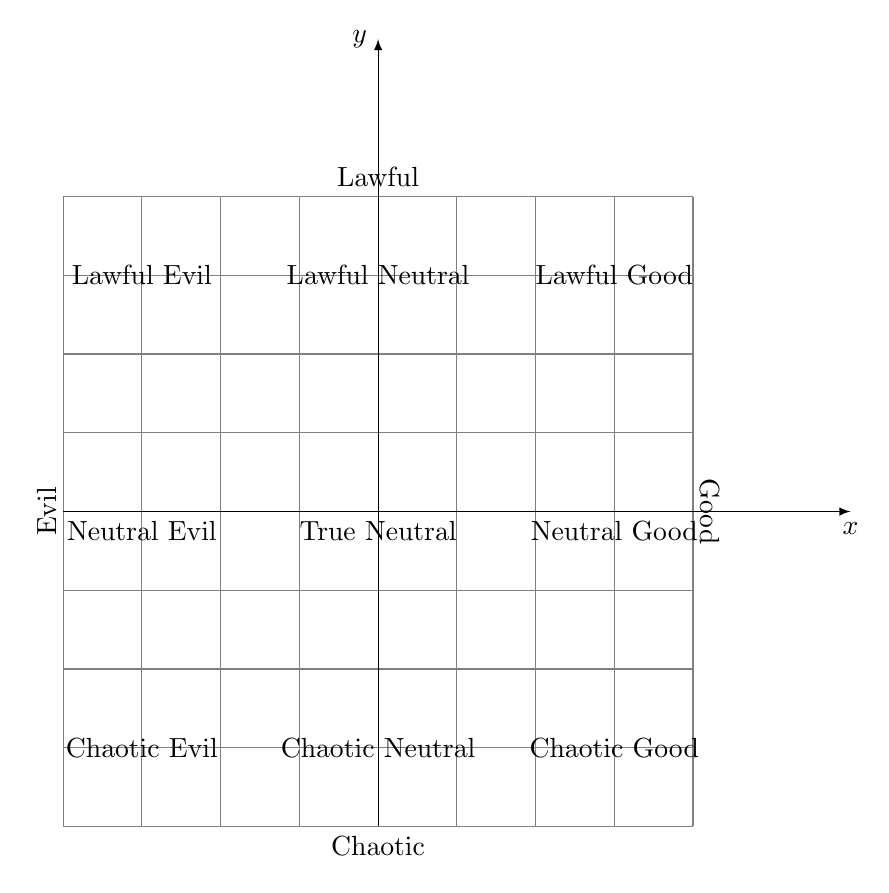
\begin{tikzpicture}
  \begin{scope}[x=4cm, y=4cm]
    \tkzInit[xmax=1,ymax=1,xmin=-1,ymin=-1]
  \tkzGrid
          \tkzDrawX[step=0.1]
        \tkzDrawY[step=0.1]
        \tkzLabelX[orig=false,label options={font=\tiny},step=0.33]
        \tkzLabelY[orig=false,label options={font=\tiny},step=0.33]
        \draw (0,1)  node[above]                 {Lawful}  -- (0,-1) node[below]                 {Chaotic}
          (-1,0) node[xshift=-6pt,rotate=90] {Evil} -- (1,0)  node[xshift=6pt,rotate=-90] {Good};
    \node at (-0.75,0.75) {Lawful Evil};
    \node[below] at (-0.75,0) {Neutral Evil};
    \node at (-0.75,-0.75) {Chaotic Evil};
    \node at (0.75,0.75) {Lawful Good};
    \node[below] at (0.75,0) {Neutral Good};
    \node at (0.75,-0.75) {Chaotic Good};
    \node at (0,0.75) {Lawful Neutral};
    \node[below] at (0,0) {True Neutral};
    \node at (0,-0.75) {Chaotic Neutral};
    \end{scope}
  \end{tikzpicture}
  \caption{The alignment coordinate system, or alignment compass.}
  \end{center}
\end{figure}
Rather than a strict categorization of Good vs Neutral vs Evil and Lawful vs Neutral vs Chaotic, these two axes \textit{(Good vs Evil, Lawful vs Chaotic)} are tracked on a floating-point coordinate system, where both the X axis \textit{(Good vs Evil)} and Y axis \textit{(Lawful vs Chaotic)} go from 1.0 to -1.0, with 0.0 at both axes representing true neutrality. This is done, so that alignment shifts can be tracked. Nevertheless, to map to the classical system of 9 alignments:
\begin{itemize}
\item Lawful characters are between 1.0 and 0.33 on the lawfullness scale, Neutral characters are between 0.3325 and -0.33, Chaotic characters are between -0.33 and -1.0 on the lawfullness scale.
\item Good characters are between 1.0 and 0.33 on the goodness scale, Neutral characters are between 0.33 and -0.33, Evil characters are between -0.33 and -1.0 on the goodness scale.
\item For the sake of convenience and simplicity, at some places, I will still refer to the classical 9-alignment system, and will detail each nine of them below:
\end{itemize}
\subsection{Lawful Good}
\subsection{Neutral Good}
\subsection{Chaotic Good}
\subsection{Lawful Neutral}
\subsection{True Neutral}
\subsection{Chaotic Neutral}
\subsection{Lawful Evil}
\subsection{Neutral Evil}
\subsection{Chaotic Evil}
\section{Attributes and Vitals}
Each and every character has a number of assigned variables we call \textbf{attributes and vitals}. \textbf{Attributes} are, for the most part fixed for a character \textit{(though some events can alter them)}, but very often modified by status effects \textemdash they tend to range between 0 and 20 for playable characters, with 10 being an average value. \textbf{Vitals} on the other hand are constantly changing, and are measured against certain set maximums and minimums.\newline
\textbf{Attributes} include:
\begin{itemize}
\item \textbf{Strength:} Governs the damage of bow-type ranged weapons \textit{(strength below a certain number of certain bows results in range penalty or inability to even use the bow)} and the damage of blunt weapons. Strength also governs the efficency of unarmed combat. Outside of a combat context, strength will also govern the character's ability to lift heavy objects, affencting carrying capacity among other things. Having high strength comes with the drawback of increasing a character's need for protein, unless the character is undead.
\item \textbf{Endurance:} Governs the maximum number of hitpoints per body part, as well as the character's maximum stamina. High endurance also increases a character's resistance to diseases and poisons. Having high endurance comes with the drawback of increasing a character's need for fat, unless the character is undead.
\item \textbf{Dexterity:} Governs damage of piercing weapons like spears and bladed weapons such as swords, accuracy of ranged weapons, evasion chance, stealth, lockpicking, etc. Having high dexterity comes with the drawback of increasing a character's need for protein, unless the character is undead.
\item \textbf{Intelligence:} Governs the character's maximum \textit{mana/spellpoints} count, if the character is using Arcane Magic. Whether the character is a spellcaster or not, intelligence also governs a character's experience gain \textit{(the higher the intelligence, the faster the level-ups)}, aids the character at detecting things that seem unusual. Having high intelligence also comes with the drawback of increasing a character's need for carbohydrates, unless the character is undead.
\item \textbf{Willpower:} Governs magic resistance for all character, as well as the maximum \textit{mana/spellpoints} for characters that use Clerical Magic. While it increases the character's magic resistance as a whole, it especially increases resistance to mind control. NPCs with high willpower also tend to be resistant to bribery and seduction attempts. Unlike strength, endurance or dexterity, willpower does not come with the drawback of increasing the character's nutritional needs.
\item \textbf{Charisma:} Governs a character's ability to lead, convince, explain, seduce, and various other social interactions. Highly charismatic characters can talk monsters to death, while characters with low charisma will be forced to rely on favors, money or brute strength to get what they want. For characters that use Arcane Magic, Charisma governs their ability to use spells that contradict their alignment, such as Good characters using Dark Magic and Evil characters using Light Magic, with Arcane Magic users that have high Charisma having no penalties from using opposite-alignment spells. Unlike strength, endurance or dexterity, charisma does not come with the drawback of increasing the character's nutritional needs, but a disproportionate number of negative status effects reduce charisma.
\end{itemize}
\textbf{Vitals} include:
\begin{itemize}
\item \textbf{Hitpoints:} Represents how much damage the character can still sustain, unlike all the other vitals, hitpoints are counted separately for each body part of the character. Reaching zero hitpoints on vital body parts means death.
\item \textbf{Mana:} Relevant only to spellcasting character, it determines how much magical power they have left and can use to cast spells. Running out of mana means not being able to cast spells until they recover their mana via either resting or drinking mana potions.
\item \textbf{Protein:} The amount of protein in the character's system, expressed in grams. The character's need for protein is governed by their race, sex, strength and dexterity. Having under 50\% of their protein need causes the character's strength and dexterity to degrade linearly. \textbf{This vital is inactive for undead characters.}
\item \textbf{Carbohydrate:} The amount of carbohydrates in the character's system, expressed in grams. The character's need for carbohydrates is governed by their race, sex and intelligence. Having under 50\% of their carbohydrate need causes the character's intelligence to degrade linearly. \textbf{This vital is inactive for undead characters.}
\item \textbf{Fat:} The amount of fat in the character's system, expressed in grams. The character's need for fat is governed by their race, sex and endurance. Having under 50\% of their fat need causes the character's endurance to degrade linearly. \textbf{This vital is inactive for undead characters.}
\item \textbf{Calories:} Total calories in the character's system. Effectively \[(other+(4*protein)+(4*carbohydrate)+(9*fat))\], since each gram of protein is 4 calories, each gram of carbohydrates is 4 calories, and each gram of fat is 9 calories. Other calories can include every other sources of calory, but among them is chiefly alcohol, with each gram of alcohol being 7 calories. \textbf{This vital is inactive for undead characters} \textemdash otherwise, a character that reaches zero calory count starves to death. Overeating has negative consequences, like temporarily reducing dexterity and charisma.
\item \textbf{Alcohol:} The amount of alcohol in the character's system, expressed in blood alcohol content \textit{(a percentage of ethanol in the blood in units of mass of alcohol per volume of blood)}, primarily to determine the character's level of intoxication. \textbf{This vital is inactive for undead characters} \textemdash otherwise, blood alcohol content above 0.500 is lethal \textit{(death by alcohol poisoning)}, blood alcohol content between 0.500 and 0.029 equates to varying levels of drunkenness, and blood alcohol content below 0.029 has no symptoms \textit{(the character is for all intents and purposes sober)}.
\item \textbf{Water:} The hydration level of your character \textemdash unlike other counters, it is more like a timer that gets reset to 3.0 when the character is hydrated. \textbf{This vital is inactive for undead characters} \textemdash otherwise characters die of dehydration when their water level reaches zero.
\item \textbf{Blood:} The amount of foreign blood in the character's system. For vampires and theriantropes, the need for blood replaces the need for nutrients like protein, carbohydrates, fat, calories and water \textemdash as such \textbf{this vital is only active for vampires and theriantropes.}
\item \textbf{Energy:} Effectively how un-sleepy the character is. This one is active even for undead characters, since all sentient beings need rest \textemdash if not physical, then mental. It slowly and gradually depletes over time \textit{(but depletes faster when the character is doing physically or mentally demanding work)}, and is regenerates very fast by sleeping \textit{(eight hours is enough to recover 100\% of a character's energy, no matter how depleted it was)} and also by consuming certain potions or beverages  \textit{(such as black tea)}. When it is depleted, the character spontaneously faints and falls asleep. When it is near depletion, the character is supposed to feel very drowsy and even experience episodes of microsleep and general confusion.
\end{itemize}
\section{Sex}
This attribute of the character determines the character's \textbf{biological sex}, regardless of what they identify with. For the majority of races, there are only two biological sexes: male and female. However, for some races, there may be more than that, or even no sexes at all \textit{(for races that rely on asexual reproduction)}.\newline
Depending on the race, certain sexes may come with certain advantages or disadvantages \textemdash for example, human males tend to be stronger \textit{(higher strength and endurance)}, while human females tend to be more nimble and intricate \textit{(higher dexterity and charisma)}.
For NPCs, their sex will typically also, to a certain extent determine their behaviour. Among other things, unless explicitly defined as homosexual or bisexual \textit{(or under the influence of either magical mind-control or a character with exceptionally high charisma)}, NPCs will typically be immune to seduction attempt by members of their own sex.
\section{Race}
A character's \textbf{race} determines quite a lot of things about a character \textemdash their expected appearence, the number of sexes they can \textit{"choose from"}, the maximums and minimums for the various attributes, the number of body parts they have \textit{(each body part has its own counter of health points)}, etc. Some backgrounds are restricted to certain races.\newline
Characters may also have a secondary race, which is typically something they assumed during their life, while their primarily race is what they were born as. For example, for a vampire who was born a human, their primary race would be Human, with their secondary race being Vampire.\newline
Races also have a variable called an \textbf{ageing factor}, which determines how long is the typical lifespan of a race compared to humans. When calculating a character's biological age in days \textemdash so long as the character is older than 6574.5 days \textemdash we must take their chronological age, reduce it by 6574.5, divide by the race's ageing factor, then increment by 6574.5. In other words: \[\frac{chronologicalAge-6574.5}{ageingFactor}+6574.5\]
It is recommended for programmers to implement secondary races dynamically generating them from primary races and having a pointer variable to the parent race. 
\section{Background}
Unlike in other roleplaying games, there are no classes - however, instead of them, there are character backgrounds, which impose far lesser limitations on characters than classes would in classic roleplaying systems. They typically grant the characters bonus feats, a number of feats to choose at the start, bonus attributes, and various other potential bonuses - but also maluses: most backgrounds also reduce some attributes, slow down experience gain, and some may even forbid certain select feats. Some backgrounds may also grant unique feats that cannot be achieved without that background. Additionally, backgrounds also control starting money and equipment.\newline
Classical classes can be emulated via so-called \textit{"builds"}, which are optional instructions and character templates.
\section{Items, Equipment and Inventory}
Each character has an \textbf{equipment} and an \textbf{inventory}. The earlier is the a map of equipment slots and \textbf{items} equipped on those respective slots, while the latter is a list of items that the character is currently carrying, but not wearing or using.\newline
Items include weapons, clothing, armour, currency, food, beverages, potions, keys, books, scrolls, and various other articles of tangible personal property. A character's weight-carrying capacity depends on their endurance, while their maximal inventory capacity depends on equipped items, such as backpacks and bags. Equipment slots include:
\begin{itemize}
\item \textbf{Hands:} Most races have two, though some may have more, or none at all. Some negative status effects may also reduce their numbers for each characters, like for a human whose left hand was cut off. Weapons and shields occupy hands. Some weapons \textemdash the majority of ranged weapons for example \textemdash may occupy two hands at once. The hands may be occupied by various other items too, such as instruments of work or music.
\item \textbf{Fingers:} Their number depends on the number of hands, and the race's number of fingers per hand, with most races having five fingers per hand. Potentially occupied by rings. All fingers belonging to a hand may also be occupied by gloves or gauntlet.
\item \textbf{Head:} Occupied by potentially multiple stacking layers of headwear \textit{(for example, a gambeson cap, combined with a chainmail coif, and finally a bascinet)}.
\item \textbf{Face:} Occupied by potentially multiple stacking layers of jewelry that can cover the face, the ears, mouth, etc.
\item \textbf{Torso:} Occupied by potentially multiple stacking layers of clothing or armour \textit{(for example, an undershirt at the bottom, followed by a gambeson, then chainmail, and finally a breastplate)}.
\item \textbf{Shoulders:} Potentially occupied by pauldrons.
\item \textbf{Arms:} Potentially occupied by jewelry \textit{(such as torcs)} or protective armbands.
\item \textbf{Neck:} Potentially occupied by jewelry \textit{(such as necklaces or torcs)}.
\item \textbf{Legs:} Occupied by potentially multiple stacking layers of clothing or armour \textit{(for example, a loincloth at the bottom, followed by a pants, then chainmail and some leg-protecting plates)}.
\item \textbf{Feet:} Occupied by potentially multiple stacking layers of clothing or armour \textit{(for example, socks followed by boots)}.
\item \textbf{Back:} Capes or backpacks. The earlier are purely aesthetic \textit{(and can potentially impede movement)}, while the latter increase carryweight/inventory capacity.
\end{itemize}
\subsection{Weapons}
Weapons are tools occupying the hands that are used to inflict damage on hostile combatants. They come in many flavours: one-handed and two-handed, ranged and melee, primitive and complex. In the World of Artograch system, each weapon can inflict multiple different types of damage simultaneously. To sum it all up, a weapon's attributes include:
\begin{enumerate}
  \item \textbf{Handedness:} Whether the weapon can be physically wielded in one hand or not. For all intents and purposes, \textit{hand-a-half swords / bastard swords} will be classified as one-handed, even if they aren't very practical for one-handed use by weaker swordsmen. The majority of ranged weapons are two-handed.
  \item \textbf{Rangedness:} Whether the weapon is a melee weapon or a \textit{ranged weapon / projectile-based weapon}.
  \item \textbf{Group:} In addition to the previous four potential groups, \textit{(one-handed, two-handed, melee, projectile)}, a weapon can be part of various other groups as well. Think of it as a tag. This is primarily used to keep track of which kind of weapons do the various feats augment. Modules can introduce whole new weapon groups and corresponding feats.
  \item \textbf{Damage:} A list of damages the weapon applies to its targets. Do keep in mind that most weapons simultaneously apply two kinds of damage, albeit at a different ratio.
\end{enumerate}
\subsection{Armour}
Armour occupies various parts of the body, and can often be combined to constitute multiple stacking layers. The primary goal of armour is to provide resistance against attacks, primarily physical ones \textit{(tho enchanted armour may offer magic resistance)}. If we assume that a character's outfit - excluding jewellry - consists of a maximum of 6 \textit{slots/layers} \textit{(underwear, shirt, sweater, coat or gambeson, chainmail or leather armour, and finally a breastplate)}, then we can neatly divide types of armour into these main categories:
\begin{itemize}
\item \textbf{Gambeson:} Occupying the fourth outfit slot, it is effectively a padded jacket, it doubles as both a piece of armour and a winter coat, protecting its user from slashing damage and cold thermal damage. It doesn't offer much resistance against piercing and crushing damage. Gambeson is typically worn under other types of armour, thus combined with leather armour, chainmail, plate mail, etc.
\item \textbf{Leather Armour:} Occupying the fifth outfit slot, it is boiled and hardened leather processed into a piece of armour, it is typically worn over a gambeson, providing additional protection.
\item \textbf{Chainmail:} Occupying the fifth outfit slot, it is a series of metal chains linked together, it is pretty much always worn over a gambeson, augmenting it with resistance against slashing damage.
\item \textbf{Scalemail:} Occupying the fifth outfit slot, also known as \textbf{Lamellar Armour}, it is a type of body armour, made from small rectangular plates \textit{(scales or \textbf{lamellae})} of iron, leather \textit{(rawhide)}, or bronze laced into horizontal rows; it is pretty much always worn over a gambeson, augmenting it with resistance against slashing damage, and to a lesser extent, piercing damage.
\item \textbf{Breastplate:} Occupying the sixth outfit slot, it is typically multiple joined solid metal pieces - plates - that wrap around the wearer's chest, it offers protection against both slashing and piercing damage. It is typically worn over chainmail, or at the very least gambeson.
\item \textbf{Platemail:} Occupying both the fifth and sixth outfit slots, it is similar to a breastplate, but expanded to cover the whole body. A full suit of plate armour offers good protection against both piercing and crushing damage. It is always worn above a gambeson.
\end{itemize}
\section{Feats}
\textbf{Feats} encapsulate the character's learned skills. Some feats give the character special abilities, some give mundane bonuses, while others may be necessary to commit certain actions \textit{(either commit them at all, or commit them without serious penalties)}. Most backgrounds give character certain starting feats. Some feats may be unique to certain backgrounds, or disallowed for certain backgrounds.
\section{Spells}
For characters that rely on magic, \textbf{spells} are powers, abilities and incantations that the spellcaster can rely on for all kinds of purposes, such as healing a wounded ally, damaging enemies, or even completely mundane things, like making menial labour less demanding. In the World of Artograch universe, magic is subdivided by two dimensions. The first being the question whether it is Arcane or Clerical:
\begin{itemize}
\item \textbf{Arcane Magic}, also known as \textit{Profane Magic} is the type of magic utilized by Magicians, Warlocks, Witches and Wizards. This kind of magic utilizes the powers of the spellcaster itself, relying on no aid from deities. Maximum mana depends on the character's Intelligence attribute. When low on mana, the character can use a forbidden technique to consume their own life force or calories to fuel their mana. Arcane Magic tends to influence its spellcaster in various ways, with Dark Magic being known for being an addictive and corrupting influence on its user. Arcane Magic is also known for taking its toll on the spellcaster's physical body.
\item \textbf{Clerical Magic} is the type of magic where the character is granted their powers from the deities they worship, making their magic partially faith-fueled. This comes with both advantages and disadvantages. On the positive side, Clerical Magic does not take its toll on the user, and allows mana to regenerate even during battle \textemdash additionally, while spells can still be learned via books and scrolls, users of Clerical Magic have a tendency to spontaneously learn new spells out of nowhere. On the negative side, their selection of spells is limited by their religion and alignment \textit{(Clerics affiliated with a Light-oriented religion are limited to healing, anti-undead and anti-demonic spells, for example, with very limited destructive capabilities against foes of other types)}, and they cannot consume their own life forces or calories to regenerate mana. For users of Clerical Magic, their maximal mana depends on their Willpower attribute. To compensate for the limited \textemdash if not nonexistent \textemdash repertoire of destructive spells, users of Clerical Magic tend to compensate by also being capable warriors, especially skilled at melee combat. 
\item \textbf{Nature Magic} is a subvariant of Clerical Magic used by Druids and Rangers, who draw their powers from the \textit{"forces of nature"} as much as they do from their deities: they absorb magical energies while doing deeds the favour nature, such as planting trees, taking care of flowers and feeding wild animals. Another trait of Nature Magic is that it also has the diversity that Arcane Magic has, rather than being limited to a certain category of spells. Druidic Magic also comes with an impressive roster of unique spells that either allow the spellcaster to take the shape of a wild animal or to harness the power of nature by turning the wilderness against the enemy.
\end{itemize}
The other dimension would be the nature of each individual spell itself:
\begin{itemize}
\item \textbf{Basic Spells:} Spells that literally every single spellcaster possesses, without exceptions. This school of magic contains only three spells: Telekinessis \textit{(moves objects and living creatures alike, can be used to move the caster itself, with other potential uses being pushing, pulling, choking, levitation, etc.)}, Lighting \textit{(illuminating dark areas)} and Energy Bolt \textit{(a bolt or arrow composed of nothing but magical energy, the damage inflicted ranging anywhere from harmless to completely lethal, depending on the power of the spellcaster)}.
\item \textbf{Light Magic:} focuses on healing wounds, curing diseases, uncursing people and items alike, blessing people, this school of magic only has a limited roster of spells of destructive nature: the destruction \textit{(or scaring away of)} of undead and demons.
\item \textbf{Dark Magic:} focuses on bringing pain and misery upon the enemy, curses, diseases, poisons, resurrection of the dead by unholy means \textit{(necromancy)}, just like Light Magic, Dark magic only has limited amount of spells that really do cause direct damage, and they often do via slow and cruel means, such as blight and strangulation.
\item \textbf{Elemental Magic:} Making use of the elements, Elemental Magic is usually divided in two or four categories, depending on the school of thought. Some prefer subdividing it into Destruction Magic and Summoning Magic \textit{(the names speak for themselves)}, while others prefer subdividing it based on the four elements \textit{(Earth Magic, Air Magic, Fire Magic, Water Magic)}.
\item \textbf{Utility Magic:} Containing various other spells that cannot be categorized into any of the aforementioned schools of magic, such as spells that aid Lockpicking, spells that lock doors magically, Teleportation, etc. Out of the three Basic Spells, Telekinessis and Lighting can be considered examples of Utility Magic.
\end{itemize}
\section{Status effects}
\textbf{Status effects} encapsulate the various modifiers affecting the character, be it passive and unnoticeable, or active, temporary and very much visible. Status effects influence the character's attributes, strengthen or weaken magic used by the character, disable certain equipment slots, influence the character's combat capabilities \textit{(some negative status effects render a character temporarily unable to act at all, forcing them to skip turns until the status effect is removed)}.
\section{Body parts}
In the World of Artograch RPG, each and every \textbf{body part} has its own health meter. When that health meter is depleted, bad things can happen: if we're talking about a limb, the character is imparted with a negative status effect and certain equipment slots are bound to be disabled \textemdash if the body part in question is not a limb, then the depletion of its health points causes death \textit{(or unconsciousness, if house rules rule out death)}, as the vital body part in question is assumed to be destroyed.\newline
The exact number of body parts a character can have depends on their race, though most humanoid races have one head, one torso, two arms and two legs, out of which the head and the torso are vital, with depletion of its hitpoints causing death - while loss of arms and legs merely disables the corresponding inventory slots.\newline
The fact that each body part has its own health meter is one of the reasons why the World of Artograch roleplaying system is not recommended for actual tabletop roleplaying \textit{(in spite of technically being possible)}, but rather is intended to serve as the basis of computer-based adaptations.\newline
As most humanoid races have a single torso, a single head, two arms and two legs, below will be shown the health scaling for those body parts:\newline
\begin{tabular}{|c|c|c|c|c|c|}
\hline
\textbf{Torso} & \textbf{Head} & \textbf{Left Arm} & \textbf{Right Arm} & \textbf{Left Leg} & \textbf{Right Leg} \\ \hline
$\frac{\textit{Base HP\ast}}{1} $ & $ \frac{\textit{Base HP\ast}}{4} $ & $ \frac{\textit{Base HP\ast}}{5} $ & $ \frac{\textit{Base HP\ast}}{5} $ & $ \frac{\textit{Base HP\ast}}{2} $ & $ \frac{\textit{Base HP\ast}}{2} $ \\ \hline
\end{tabular}\newline
$ \textbf{\ast Base HP} $ is the character's $ \textbf{Endurance} \cdot 10 $, unless there are some other modifiers at play, such as status effects or feats. In other words, without any other modifiers, a typical humanoid character with an Endurance of 10 will have a torso with $ \frac{10 \cdot 10}{1} = 100 $ HP, a head with $ \frac{10 \cdot 10}{4} = 25 $ HP, a right arm and a left arm each with $ \frac{10 \cdot 10}{5} = 20 $ HP, and finally a right leg and a left lef each with $ \frac{10 \cdot 10}{2} = 50 $ HP.\newline
Chances to hit a certain body part also scale with the amount of maximum HP each body part can potentially have: if we add together 100, 25, 20, 20, 50 and 50, we get 265, which results in ratios of $ \frac{100}{265}=37.73\% $, $ \frac{25}{265}=9.43\% $, $ \frac{20}{265}=7.55\% $, $ \frac{20}{265}=7.55\% $, $ \frac{50}{265}=18.88\% $ and $ \frac{50}{265}=18.88\% $ respectively. But what does that exactly mean? It means that if the character simply attacks the enemy without targetting any particular body part, we generate a random number between 0 and 100, and then, if the number is is above 81, it is the right leg - if it's below that, but still above 62, it's the left leg, right arm if below that but above 55, left arm if below that but above 47, head if below that but above 38, and torso if below 38 - alternatively, in a more simplifeid dice-rolling system, one most use two 10-sided dice or four 5-sided dice, and the numbers are instead 16, 12, 11, 9, 8.\newline
If the attacker is attacking from a mount, the legs cannot be targeted and will never be hit, which means that the numbers should instead be $ \frac{100}{165}=60.60\% $, $ \frac{25}{165}=15.15\% $, $ \frac{20}{165}=12.12\% $, $ \frac{20}{165}=12.12\% $ - that is, above 88 for right hand, below that but above 76 for left hand, below that but above 61 for head, and below 61 for torso; with the numbers instead being 18, 15 and 12 for dice-rolling.
\end{document}
